\documentclass[english,notitlepage]{revtex4-1}  % defines the basic parameters of the document
%For preview: skriv i terminal: latexmk -pdf -pvc filnavn



% if you want a single-column, remove reprint

% allows special characters (including æøå)
\usepackage[utf8]{inputenc}
%\usepackage[english]{babel}

%% note that you may need to download some of these packages manually, it depends on your setup.
%% I recommend downloading TeXMaker, because it includes a large library of the most common packages.

\usepackage{physics,amssymb}  % mathematical symbols (physics imports amsmath)
\include{amsmath}
\usepackage{graphicx}         % include graphics such as plots
\usepackage{xcolor}           % set colors
\usepackage{hyperref}         % automagic cross-referencing (this is GODLIKE)
\usepackage{listings}         % display code
\usepackage{subfigure}        % imports a lot of cool and useful figure commands
\usepackage{float}
%\usepackage[section]{placeins}
\usepackage{algorithm}
\usepackage[noend]{algpseudocode}
\usepackage{subfigure}
\usepackage{tikz}
\usetikzlibrary{quantikz}
% defines the color of hyperref objects
% Blending two colors:  blue!80!black  =  80% blue and 20% black
\hypersetup{ % this is just my personal choice, feel free to change things
    colorlinks,
    linkcolor={red!50!black},
    citecolor={blue!50!black},
    urlcolor={blue!80!black}}

%% Defines the style of the programming listing
%% This is actually my personal template, go ahead and change stuff if you want



%% USEFUL LINKS:
%%
%%   UiO LaTeX guides:        https://www.mn.uio.no/ifi/tjenester/it/hjelp/latex/
%%   mathematics:             https://en.wikibooks.org/wiki/LaTeX/Mathematics

%%   PHYSICS !                https://mirror.hmc.edu/ctan/macros/latex/contrib/physics/physics.pdf

%%   the basics of Tikz:       https://en.wikibooks.org/wiki/LaTeX/PGF/Tikz
%%   all the colors!:          https://en.wikibooks.org/wiki/LaTeX/Colors
%%   how to draw tables:       https://en.wikibooks.org/wiki/LaTeX/Tables
%%   code listing styles:      https://en.wikibooks.org/wiki/LaTeX/Source_Code_Listings
%%   \includegraphics          https://en.wikibooks.org/wiki/LaTeX/Importing_Graphics
%%   learn more about figures  https://en.wikibooks.org/wiki/LaTeX/Floats,_Figures_and_Captions
%%   automagic bibliography:   https://en.wikibooks.org/wiki/LaTeX/Bibliography_Management  (this one is kinda difficult the first time)
%%   REVTeX Guide:             http://www.physics.csbsju.edu/370/papers/Journal_Style_Manuals/auguide4-1.pdf
%%
%%   (this document is of class "revtex4-1", the REVTeX Guide explains how the class works)


%% CREATING THE .pdf FILE USING LINUX IN THE TERMINAL
%%
%% [terminal]$ pdflatex template.tex
%%
%% Run the command twice, always.
%% If you want to use \footnote, you need to run these commands (IN THIS SPECIFIC ORDER)
%%
%% [terminal]$ pdflatex template.tex
%% [terminal]$ bibtex template
%% [terminal]$ pdflatex template.tex
%% [terminal]$ pdflatex template.tex
%%
%% Don't ask me why, I don't know.

\begin{document}

\title{Title of the document}      % self-explanatory
\author{Henrik Modahl Breitenstein}          % self-explanatory
\author{Carl Petter Duedahl}
\date{\today}                             % self-explanatory
\noaffiliation                            % ignore this, but keep it.


\maketitle

\begin{center}
	\textit{https://github.com/henrikbreitenstein/FYS3150.git}
\end{center}

\section*{Problem 1}

Poisson likningen
$$- \frac{\mathrm{d}^2 u}{\mathrm{d}x^2} = f(x)$$

Bytter $f(x)$ med gitt funksjon

\begin{align*}
- \frac{\mathrm{d}^2 u}{\mathrm{d}x^2} =& 100e^{-10x} \\
-\mathrm{d}^2 u =& 100e^{-10x} \; \mathrm{d}x^2
\end{align*}
Tar integralene

\begin{align*}
-\iint \mathrm{d}^2 u =& \iint 100e^{-10x} \; \mathrm{d}x^2 \\
-u =& \int -10e^{-10x} + c_1 \; \mathrm{d} x \\
-u =& e^{-10x} + c_1x + c_2 \\
u =& -e^{-10x} - c_1x - c_2 \\
\end{align*}
Bruker initialbetingelsene


\begin{equation}\label{eq1}
u(0) = 0 \Rightarrow - 1 - c_2 = 0
\end{equation}


\begin{equation}\label{eq2}
u(1) = 0 \Rightarrow -e^{-10} -c1 -c2 = 0
\end{equation}

Med \ref{eq1} og \ref{eq2} får vi:

\begin{align*}
c2 =& -1 \\
c1 =& 1 - e^{-10}
\end{align*}
Ved å sette inn for $c_1$ og $c_2$ får vi:

\begin{equation}\label{equ}
u = 1 - (1-e^{-10})x - e^{-10x}
\end{equation}


\section*{Problem 2}

I repostory'et under FYS3150/Project1/main.cpp så har vi skrevet koden som regner ut verdiene til den eksakte løsningen, og i FYS3150/Project1/plot.py så tegnes grafen. Kan kjøre programmet 'main.cpp' med commandoen \\

\$ make all

og kjøre 'plot.py' med \\

\$ python plot.py

\section*{Problem 5}
\subsection*{Problem a}

Siden vi gjør en matrismultiplikasjon så må bredden, $n$, til $\textbf{A}$ være det samme som lengden $m$ til $\overrightarrow{v}$ og $\overrightarrow{g}$. Så

$$n = m$$

\subsection*{Problem b}
Av $A\vec{v}=\vec{g}$ vil vi finne alle verdier mellom grensebetingelsene $u(0)=u(1)=0$. $\vec{v*}$ er den samme som $\vec{v}$ men vi har lagt til $v_0$ og $v_{n+1}$ som er grensebetingelsene.

\section*{Problem 6}

\section*{a}
Vi har nå en vektor
$$
\vec{v}=\begin{pmatrix}
v_1 \\ v_2 \\ \vdots \\ v_n
\end{pmatrix}
$$
og en $n\cross n$-matrise
$$
\textbf{A}=\begin{Bmatrix}
b_1 & c_2 & 0 & 0 & \cdots & 0 &0 \\
a_2 & b_2 & c_2 & 0 & \cdots &0 &0 \\
0 & a_3 & b_3 & c_3 & \cdots & 0 &0 \\
\vdots & \vdots&\vdots&\vdots&\ddots & \vdots & \vdots\\
0& \cdots &  \cdots&\cdots&\cdots& a_n & b_n
\end{Bmatrix}
$$
Matrisemultipliserer vi disse får vi
$$
\textbf{A}\vec{v}=
\begin{matrix}
(I)&b_1 v_1 &+ c_1 v_2 & &&=g_1 \\
(II) &a_2 v_1&+b_2v_2&+c_3 v_3 &&=g_2\\
(III)& & a_3v_2 &+b_3v_3 &+ c_3 v_4 &=g_3\\
\vdots&&&&&\\
(n)&&&a_n v_{n-1}&+b_n v_n&=g_n\\

\end{matrix}
$$ Herfra skal vi radredusere og starter med å ta $(II)-\frac{a_2}{b_1}(I)$ slik at vi får $$\begin{matrix}
(II*) & 0&b_2-\frac{c_1\cdot a_2}{b_1}& c_2 &\cdots & g_2-g_1\frac{a_2}{b_1}
\end{matrix}$$
og vi ser da at $a_2$ går bort. Vi kan også sette $b_2^*\equiv b_2-\frac{a_2 \cdot c_1}{b_1}$ og $g_2^*\equiv g_2-g_1\frac{a_2}{b_1}$. Da har vi mellom $(II^*)$ og $(III)$ noe som ser ganske likt ut som det vi hadde mellom $(I)$ og $(II)$. Derfor gjør vi det samme som vi gjorde før og tar $(III)-\frac{a_3}{b_2^*}(II)^*$ og får
$$
\begin{matrix}
(III)^* & 0 &0& b_3-\frac{c_2\cdot a_3}{b_2^*}&c_3 & g_3-g_1\frac{a_3}{b_2^*}
\end{matrix}
$$
og vi kan igjen definere $b_3^*=b_3-\frac{c_2\cdot a_3}{b_2^*}$ og $g_3^*=g_3-g_1\frac{a_3}{b_2^*}$. Og vi kan da fortsette med dette nedover som $(k)-\frac{a_{k}}{b_{k-1}^*}(k-1)^*$. Så har vi fjernet $a$-ene så da må vi fjerne $c$-ene og normalisere b-ene. For å gjøre starter vi i siste ledd med

$$
(n)/b_n
$$
så
$$
b_n=\frac{b_n}{b_n}
$$
og
$$
g_n^*=\frac{g_n}{b_n}
$$
Da får vi at
$
A_n v_n=g_n
$
blir satt ned til
$$
v_n=\frac{g_n}{b_n}
$$

$$
\begin{matrix}
(n-1)^* & 0& \cdots & b_{n-1}^* &c_{n-1}&g_{n-1}^* \\
(n)^* & 0 & \cdots & 0 & b_{n}^*& g_{n-1}^*
\end{matrix}
$$
så hvis vi da tar $(n-1)^*-\frac{c_{n-1}}{b_n^*}(n)^*$ får vi
$$
\begin{matrix}
\tilde{(n-1)} & 0 & \cdots & b_{n-1}^* & 0 & g_{n-1}^*-\frac{c_{n-1} g_n^*}{b_n^*}
\end{matrix}
$$
og vi setter $\tilde{g_{n-1}}= g_{n-1}^*-\frac{c_{n-1} g_n^*}{b_n^*}$ og dette gjør vi videre oppover som $(k-1)-\frac{c_k}{b_{k-1}}(k)$
Til slutt står vi da bare igjen med $b^*$-ene og disse kan vi da dele på seg selv og vi får en identitetsmatrise.
Vi kan nå skrive dette som en algoritme. Anta vi har en tridiagonal matrise
$$
A=U=\begin{pmatrix}
u_{1,1}&u_{1,2}&\cdots & u_{1,n} \\
u_{2,1}&u_{2,2}&\cdots & u_{2,n} \\
\vdots & \vdots& \ddots & \vdots \\
u_{n,1} & u{n,2}& \cdots & u{n,n}
\end{pmatrix}
$$
og en som skal løses for vektoren
$$
g=h=\begin{pmatrix}
h_1\\h_2\\\vdots \\ h_n
\end{pmatrix}
$$

\begin{algorithm}[H]
	\caption{Radredusering av tridiagonal matrise}\label{algo:midpoint_rule}
	\begin{algorithmic}
		\For{$i = 2, 3, ..., n$} \Comment{Forward substitution, $n-1$ repetisjoner}
		\State $$t\leftarrow \frac{u_{i,i-1}}{u{_i-1,i}}$$ \Comment{1 FLOP}
		$$
		u_{i,i-1}\leftarrow u_{i,i-1}-u_{i-1,i-1} \cdot t
		$$ \Comment{2 FLOPs}
		$$
		u_{i,i}\leftarrow u_{i,i}-u_{i-1,i-1}\cdot t
		$$ \Comment{2 FLOPs}
		$$
		h_i\leftarrow h_i-h_{i-1} t
		$$ \Comment{2 FLOPs} \\
		\EndFor
		\Comment{Til sammen $7\cdot (n-1)$ FLOPs i loopen}
		\For{$j=n-1,n-2, ... ,1$} \Comment{Backward Substitution, $n-1$ repetisjoner}
		\State $$k\leftarrow \frac{u_{j,j+1}}{u_{j+1,j}}$$ \Comment{2 FLOPs}
		$$
		u_{j,j+1}\leftarrow u_{j,j+1}-u_{j+1,j+1}\cdot k
		$$ \Comment{2 FLOPs}
		$$
		u_{j,j}\leftarrow u_{j,j}-u_{j+1,j}\cdot k
		$$ \Comment{2 FLOPs}
		$$
		h_j\leftarrow h_j-h_{j+1}\cdot k
		$$ \Comment{2 FLOPs} \\
		\EndFor
		\Comment{Til sammen $7\cdot (n-1)$ FLOPs i loopen}
		\For {$l=1,2,\cdots n$} \Comment{Deler for å få identitetsmatrise, til sammen $n$ repetisjoner}
		\State $$
		u_l \leftarrow \frac{u_l}{u_l}$$ \Comment{1 FLOP}
		$$
		h_l\leftarrow \frac{h_l}{u_l}
		$$ \Comment{1 FLOPs} \\
		\EndFor
		\Comment{Til sammen $2\cdot n$ FLOPs}
	\end{algorithmic}
\end{algorithm}
Da ser vi at vi til sammen får $2\cdot n+ 2\cdot 7\cdot (n-1)=16n-14$ FLOPs.

\section*{Problem 7}

\subsection*{Problem a}

Sriptet 'Problem7new.cpp' og 'Problem7func.cpp' bruker den generelle algoritmen  til å løse matriselikningen. For å kjøre de sammen: \\

\$ make pr7all

\subsection*{Problem b}

Vi kjørte for $n = 10$ i \ref{7n100}, $n = 100$ i \ref{7n100} og $n = 1000$ i \ref{7n1000}. 

\begin{figure}
\centering
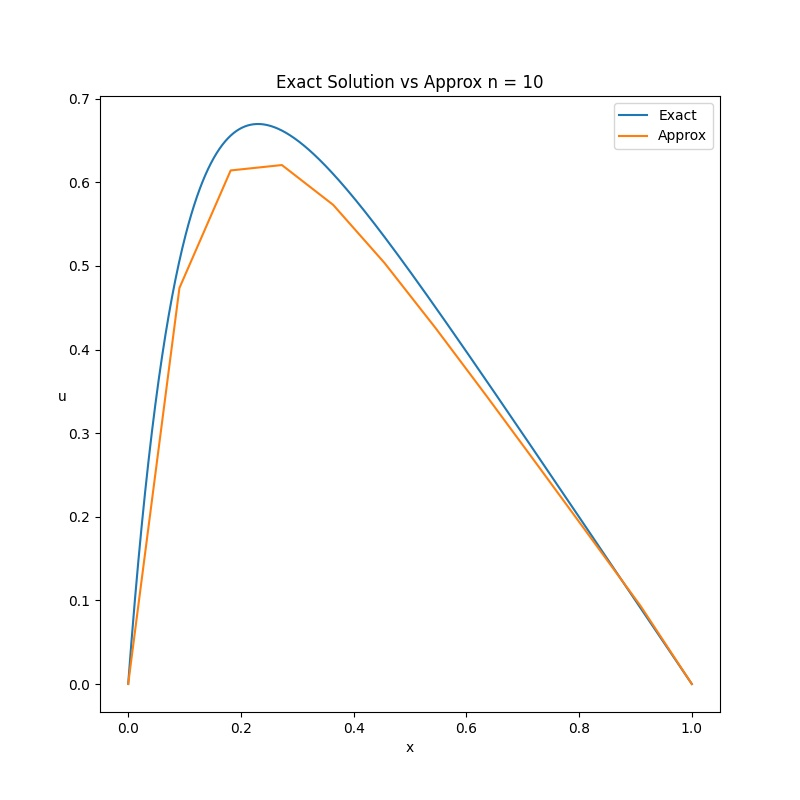
\includegraphics[scale=0.65]{Images/problem7NEW10.jpg}
\caption{Eksakt $u(x)$ og tilnærmingen $v(x)$ hvor vi har brukt $n = 10$ som antall steg.}
\label{7n10}
\end{figure}

\begin{figure}
\centering
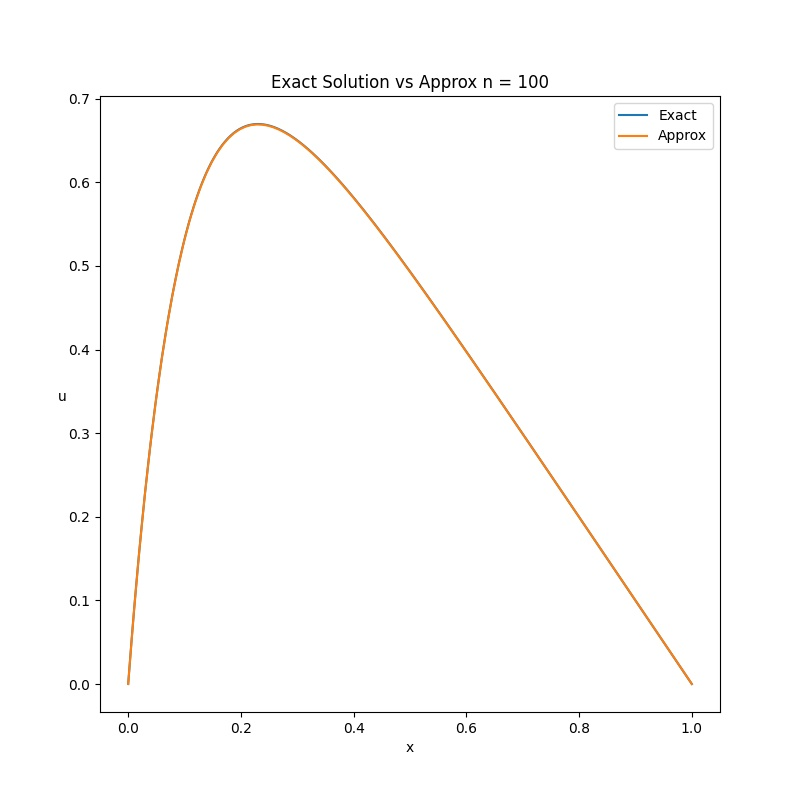
\includegraphics[scale=0.65]{Images/problem7NEW100.jpg}
\caption{Eksakt $u(x)$ og tilnærmingen $v(x)$ hvor vi har brukt $n = 100$ som antall steg.}
\label{7n100}
\end{figure}

\begin{figure}
\centering
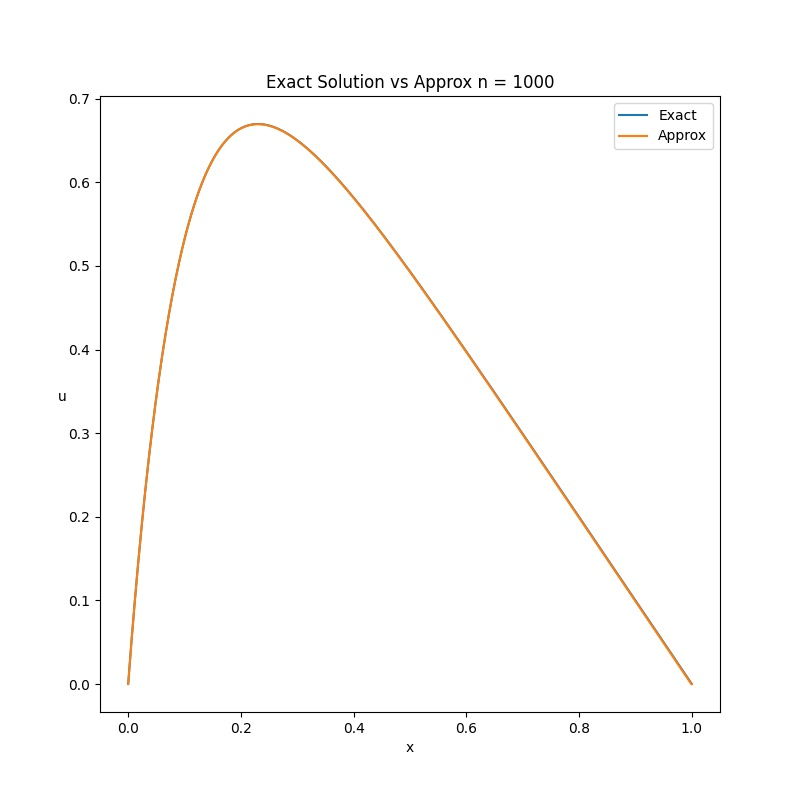
\includegraphics[scale=0.65]{Images/problem7NEW1000.jpg}
\caption{Eksakt $u(x)$ og tilnærmingen $v(x)$ hvor vi har brukt $n = 1000$ som antall steg.}
\label{7n1000}
\end{figure}

Legger merker til at etter $n = 100$ så ser man ikke den eksakte grafen lenger, og det er vanskelig å si med det blåtte øyet om tilnærmingen blir bedre eller ikke.

\section*{Problem 8}

\subsection*{Problem a}
Vi har illustrert den absolutte feilen mellom den eksakte verdien og vår tilnærming i \ref{abserr}.

\begin{figure}
\centering
\includegraphics[scale=0.65]{•}
\caption{Den absolutte feilen mellom den eksakte verdien, $u(x)$, og vår tilnærming $v(x)$.}
\label{abserr}
\end{figure}
\subsection*{problem b}
\subsection*{Problem c}

\section*{Problem 9}

\subsection*{Problem a}

\begin{algorithm}[H]
	\caption{Spesialisert algoritme}\label{algo:spec}
	\begin{algorithmic}
	\State $$a \leftarrow -1$$
	\State $$b \leftarrow 2$$
	\State $$c \leftarrow -1$$
	\State $$d \leftarrow a \cdot c$$ \Comment{1 FLOP}
	\For {$i=0, 1, 2, \cdots, n-1$} \Comment{Forward elemination}
	\State $$\widetilde{b}_{i+1} \leftarrow \widetilde{b}_{i+1} - \frac{d}{\widetilde{b}_i}$$ \Comment{2 FLOPs} \\
	\State $$\widetilde{g}_{i+1} \leftarrow g_{i+1} - \frac{a}{\widetilde{b}_i}g_i$$ \Comment{3 FLOPs} \\
	\EndFor
	\For {$i=n-1, n-2, \cdots, 0$} \Comment{Backward elemination}
	\State $$v_i \leftarrow \frac{\widetilde{g}_i - cv_{i+1}}{\widetilde{b}_i}$$ \Comment{3 FLOPs} 
	\EndFor
	\end{algorithmic}
\end{algorithm}

\subsection*{problem b}

Vi regner ut produktet $a \cdot c$ som gir oss $1$ FLOP. For "Forward Elemination" loopen så har vi 5 FLOPs per iterasjoner, som gir tilsammen $5n$. I loopen for "Backwards elemination" så har 3 FLOPs per iterasjon som gir oss $3n$ FLOPs tilsammen. Totalt ender vi da opp med $8n + 1$ FLOPs.

\subsection*{Problem c}

I filen 'problem9.cpp' har vi kodet den spesielle algoritmen. Kjøres ved kommandoen \\

\$ make p9all

\section*{Problem 10}

\section*{Problem 11}

Med LU dekomposisjon så vil man bruke i utgangspunktet $N^3$ FLOPs kun for dekomposisjonen og så skalerer kompleksiteten til å løse hver enkelt $\textbf{A}\vec{v}= \vec{g}$ likning med $N^2$. For kun én slik likningen kan vi se at både den generelle og spesielle algoritmen når man har en tridiagonal matrise skalerer to ordner lavere enn LU dekomposisjon.

\end{document}


























